\documentclass[10pt]{article}
%%%%%%%%%%%%%%%%%%%%%%%%%%%%%%%%%%%%%%%%
\usepackage{amsmath}
\usepackage{verbatim}
\usepackage[usenames,dvipsnames]{color}
\usepackage{setspace}
\usepackage{lscape}
\usepackage{longtable}
\usepackage[top=1.25in,bottom=1.25in,left=1in,right=1in]{geometry}
\usepackage{graphicx}
\usepackage{epstopdf}
\usepackage[usenames,dvipsnames]{pstricks}
\usepackage{epsfig}
\usepackage{pstricks-add}
\usepackage{pst-node}
\usepackage{pst-plot}
\usepackage{fancyhdr}
\usepackage[absolute,showboxes]{textpos}
\usepackage{booktabs}
\usepackage{dcolumn}
\usepackage{arydshln}
\usepackage{natbib}

\setcounter{MaxMatrixCols}{10}
\newcolumntype{d}[1]{D{.}{.}{-2.#1}}
\newenvironment{proof}[1][Proof]{\noindent\textbf{#1.} }{\ \rule{0.5em}{0.5em}}
\setlength{\columnsep}{.2in}
\psset{unit=1cm}

\begin{document}
\begin{titlepage}
\vspace{2in} \noindent {\large \today}

\vspace{.5in} \noindent {\Large \textbf{\strut The Influence of Crop Type on Comparative Development}}

\vspace{.25in} \noindent {\large T. Ryan Johnson}

\vspace{.05in} \noindent University of Houston

\vspace{.25in} \noindent {\large Dietrich Vollrath}

\vspace{.05in} \noindent University of Houston

\vfill \noindent \textsc{Abstract} \hrulefill

\vspace{.05in} \noindent Stuff

\vspace{.1in} \hrule

\vspace{.5in} \noindent {\small JEL Codes: TBD}

\vspace{.1in} \noindent {\small Keywords: TDB}

\vspace{.1in} \noindent {\small Contact information: 201C McElhinney Hall, U. of Houston, Houston, TX 77204, devollrath@uh.edu.}
\end{titlepage}

\pagebreak 

\section{Introduction}
\onehalfspacing

If not through agricultural productivity levels, there are two ways in which Malthusian forces could be "tighter". The first is in the elasticity of population growth with respect to living standards. TK cites

The second concept of "tightness" in a Malthusian economy is the elasticity of living standards with respect to population density, which in a textbook model would be equal to the elasticity of output with respect to the fixed factor of production (e.g. land). If that elasticity goes towards zero, then the fixed factor ceases to be a constraint and a Malthusian economy can achieve very high population densities without lowering living standards. As that elasticity gets higher, however, the fixed factor of production becomes more crucial to production, and the Malthusian constraint is "tight" in the sense that living standards are highly sensitive to population density. 

It is the second concept of Malthusian "tightness" that we explore in this paper. 

Establish that tightness varies by region, and then relate to crops


One of the closest related studies is \citet{mfm2014}. Those authors examine the growth of urbanization at the grid-cell level, specifically the timing of when grid-cells pass certain thresholds of urban population density (i.e. 5.67 urban residents per square kilometer, equivalent to 5,000 urban residents in a grid cell near the poles), or the percent of urban population in the cell. They relate the year a cell passes these thresholds to a series of geographic determinants, including distance to coast, order of streams, frost prevalance, and cultivation suitability. There is a significant correlation of urbanization with the cultivation suitability measure from \citet{ramankutty2002}. That measure, however, does not distinguish types of crops, and is solely a measure of the probability that a grid cell will be cultivated. It is not a measure of the productivity of crops, of any type, in that cell. Relative to \citet{mfm2014}, we will be looking specifically at the effect of crop productivity levels on urbanization and population density, as well as considering non-linearities and crop-level differences in the relationships.




\section{The Relationship of Productivity and Rural Density}



\subsection{The Tightness of the Malthusian Constraint}
Consider an economy that has $I$ distinct geographic sub-units in which agricultural production can take place, such as states or provinces within a given country. For each sub-unit $i$, agricultural production is
\begin{equation}
Y_{i} = A_{i} X_{i}^{\beta} (L^A_{i})^{1-\beta}
\end{equation}
where $A_{i}$ is total factor productivity, $X_{i}$ is land, and $L^A_{i}$ is the number of agricultural workers (there may be non-agricultural workers in sub-unit $i$ as well). The value of $\beta$ is assumed to be constant across the sub-units of the economy.

If workers are paid their marginal product, then for sub-unit $i$ we have a wage of
\begin{equation}
	w_{i} = p (1-\beta) A_{i} X_{i}^{\beta} (L^A_{i})^{-\beta},
\end{equation}
where $p$ is the relative price of agricultural goods, and is assumed to be the same across sub-units in the region (i.e. output is freely traded within the region). With free mobility of labor within the region, it will be that $w_{i} = w_{j}$ for any given pair of sub-units $i$ and $j$.

Combine the wage equalization condition with the adding-up condition for agricultural labor 
\begin{equation}
\sum_{i\in I} L^A_{i} = L^A,
\end{equation}
where $L_A$ is the total amount of agricultural labor in the economy, and we can solve for the allocation of agricultural labor to sub-unit $i$,
\begin{equation}
L^A_{i} = A_{i}^{1/\beta}X_{i} \frac{L^A}{\sum_{j\in I} A_{j}^{1/\beta}X_{j}}.
\end{equation}
This says that total agricultural employment in sub-unit $i$ depends on its own productivity level and area, relative to the weighted sum of productivity terms across the whole region. Intuitively, any sub-unit that is particularly productive should have a greater share of the agricultural labor force employed in it. The larger is economy-wide agricultural labor, $L^A$, the larger is agricultural labor in any given sub-uit.

Note that the fraction on the right is common to every sub-unit in the region. For notational simplicity, write this fraction as $\Omega$, and divide both sides by $X_i$ to put this in terms of rural population density, giving us
\begin{equation}
L^A_{i}/X_i = A_{i}^{1/\beta} \Omega
\end{equation}
as the expression for the agricultural population density in sub-unit $i$. Taking logs, we have
\begin{equation}
\ln L^A_{i}/X_i = \frac{1}{\beta} \ln A_{i} + \ln \Omega. \label{eq_est}
\end{equation}
This equation shows clearly that the elasticity of agricultural population density with respect to the level of produtivity is $1/\beta$, which depends on the elasticity of output with respect to the fixed factor, land.

When $\beta$ goes to zero, land becomes irrelevant to production, and the elasticity goes to infinity. All of the agricultural labor will crowd into the single sub-unit $i$ with the highest productivity level. The crowding does not lower the marginal product of workers, and so it does not pay for them to stay in low-productivity areas. This a case where the Malthusian constraint is "loose", as the marginal product of workers is not sensitive to the number of workers.

On the other hand, as $\beta$ goes to one, land becomes crucial to production, and the elasticity goes to zero. Agricultural labor will be spread equally across the various sub-units, even if there are differences in productivity. This is the case where the Malthusian constraint is "tight", as the marginal product of workers quickly declines if more workers crowd onto the available land. 

Note that "loose" and "tight" constraints refer to the size of $\beta$ and the elasticity of agricultural density with respect to productivity, but not to the absolute \textit{level} of agricultural productivity in the economy, which is embedded in the term $\Omega$. Thus we could easily have an economy with very high levels of agricultural productivity ($A_i$ are all large) but with a "tight" constraint because $\beta$ is large, and the elasticity $1/\beta$ is small. And it is possible to think of economies with low productivity ($A_i$ are low), but with a "loose" Malthusian constraint because $\beta$ is relatively small.

\subsection{Implications of Malthusian Tightness}

\section{Variation in Malthusian Tightness}

\subsection{Cross-country Evidence}
\citet{ashraf2010dynamics} provided systematic evidence consistent with the basic predictions of a Malthusian model of population and production. Their data was at the country level, and their baseline results include simple linear regressions showing a positive relationship of population density in 1500 C.E. (as well as in 1000 C.E. and 1 C.E) with both the number of years since the Neolithic agricultural revolution and a measure of agricultural productivity. This productivity measure is based on a suitability measure from \citet{ramankutty2002} and a measure of the percent of land that is arable in a country. These are combined using principal components to arrive at a single index of agricultural productivity, which is based only on agro-climatic characteristics.

Is the positive relationship between agricultural productivity and population density consistent across regions? To answer this, we divided the original Ashraf/Galor sample into regional groups: Europe, Asia, Middle East and North Africa, Sub-Saharan Africa, and the Americas.\footnote{In defining which countries belong to which regions, we deviate slightly from those authors. Russia was excluded from all regions, as it does not clearly fall into any single one. Several countries are in both our Middle East and North Africa region, as well as in the Asia region. Nothing about this initial analysis depends crucially on that definition. Sub-Saharan Africa is, as expected, Africa less the traditionally Islamic North African nations.} We then replicated the Ashraf and Galor analysis for each region separately.

The results are best seen in Figure \ref{FIG_ag_regions}, which plots log population density in 1500 CE against the residual measure of agricultural productivity after we controlled for the additional regressors used by Ashraf and Galor in their analysis. The residual for agricultural productivity from these regressions are what is plotted on the x-axis in Figure \ref{FIG_ag_regions}.\footnote{The specific controls are (log) years since the Neolithic transition, (log) absolute latitude, the mean distance to a coast or river, and the percent of land less than 100 km from a coast or river. Continent dummies were not included as they are colinear with our regions.}

What becomes immediately apparent from Figure \ref{FIG_ag_regions} is that Europe is an outlier in several respects. First, note that population density has effectively no relationship with residual productivity. Places within Europe that are more productive are not necessarily more dense, which constrasts with the three other regions plotted in the figure. For Asia, the Mideast and North Africa, and Sub-Saharan Africa, there is a distinct positive relationship conforming to the original results in Ashraf and Galor.

The small slope for Europe is indicative of a tight Malthusian constraint, and consistent with a production function that features a large land elasticity, $\beta$. In comparison, the relationship of density and productivity in the rest of the world is indicative of a relatively loose Malthusian constraint, and a relatively low land elasticity. It is 

What is also apparent from Figure \ref{FIG_ag_regions} is that the range of (residual) productivity variation within Europe is much smaller than in other regions. This is perhaps not surprising, as Europe (excluding Russia) encompasses a much smaller physical area than the other regions, giving it less scope for variation in agro-climatic conditions. Note that this is not a statement about the absolute productivity of agriculture in Europe, which is generally among the highest in the entire sample. It is certainly possible that the lack of a significant relationship between productivity and density is because we simply do not see enough variation within Europe to detect it. Looking at sub-national level data will confirm that this is a robust feature of the data.

Before proceeding to the sub-national analysis, an additional set of suggestive facts regarding urbanization at the country level can be established. Figure \ref{FIG_ag_urban} plots the urbanization rate in 1500 CE, from \citet{ccp14}, against population density in 1500 CE, for the three regions where we have sufficient data. Here, we note that for Europe, higher population densities are associated with higher urbanization rates, so that the most dense countries are urbanized at the rate of 15-35\% (Belgium, the Netherlands, and Italy), while countries in Asia at the same density are less urbanized, at only 5-10\% (China, India, Japan). Countries of the Middle East are, relative to both of the other regions, more urbanized at all levels. The slope of the European relationship is relatively high, so that density and urbanization tend to go hand in hand, whereas in Asia and the Middle East high density is not necessarily associated with greater urbanization.


\subsection{Sub-national Evidence}


\textbf{Population:} The underlying population data comes from HYDE 3.1 \citep{hyde31}, and is provided at a 5 degree grid-cell resolution. The authors provide counts of total population as well as urban and rural population for each cell. These counts are derived from political administrative data at varying levels (e.g. districts, states) which are then used to assign counts to the grid-cells within the given political unit. By accessing administrative population data (e.g. censuses) at various points in time, the HYDE database provides estimates of population counts for each grid cell going back several centuries.

Because of the nature of their estimates, the grid-cell level counts are inappropriate for our purposes. The authors explain in the associated paper that they use several algorithms to smooth the population counts across grid cells based on land productivity and assumptions about the gradient of population density with respect to distance from urban centers. If we use their grid-cell population data directly, we will potentially be recovering their algorithm, and not a true estimate of the relationship of density and crop type.

Therefore, we only use their data at the level of political units, and not at the grid-cell level. We overlay political boundary data from the Global Administrative Areas project (GADM) on top of the HYDE grid-cell data, and use this to rebuild the population count data for each political boundary. Our primary level of analysis is the GADM first level, equivalent to states or provinces, but we also examine results using the second level (e.g. counties or districts) as the units of analysis. Details of the assumptions regarding the overlap of grid-cells and boundaries are given in the appendix. Given the counts of urban and rural population at the level of political units, it is straightforward to construct measures of the urbanization rate and population density. 

TK - note on differences in boundaries over time.

\textbf{Crop productivity:} Crop-specific productivity information is from the Global Agro-ecological Zones (GAEZ) project \citep{gaez}. This provides grid-cell level information on crop-specific measures of productivity. There are several dimensions of productivity that the GAEZ provides. ``Agro-climatic yield'' for a given crop indicates, given a set of assumptions regarding the level of input use and water supply, the potential yield of the crop given existing climatic conditions (e.g. temperature and length of growing period). This agro-climatic yield is then combined with information on soil and terrain constraints to produce a ``total production capacity'', measured in tonnes/ha, for a given crop. The FAO also produces a ``crop suitability index'', measured between 0 and 100, for each crop in a given grid-cell, and this depends on the climatic conditions, the soil and terrain constraints, and the chosen level of inputs and water supply.

TK - will the different productivity measures matter? Will the different input choices matter?

For our purposes, because we are focused on the long-run impact of crop types on the distribution of population and urbanization, we use the low-input and rain-fed data series from the GAEZ for our analysis. We are trying to estimate the effect of the potential for crop production in the pre-industrial era, and so these assumptions seem most appropriate. A similar choice is made in \citet{galorozak2016}. 

\textbf{Overall agricultural productivity:} We also use the work of \citet{galorozak2016} to provide one of our measures of general agricultural productivity. The authors form a measure of the potential caloric yield at a grid-cell level, combining yield information from the GAEZ with nutritional information for crops. Their measure shows the maximum possible calories that can be produced in a given grid-cell. While there is an implied crop underlying this maximum (e.g. rice may provide the most possible calories for a given grid-cell), the value of their measure is that productivity is measured in a comparable manner, using calories. What we will be examining below is, in part, whether the kind of crops involved in providing calories are as important in the number of calories in determining density and urbanization.

In addition to the calorie production measure, we also use measures of agro-climatic conditions at the grid-cell level from the GAEZ that are not crop-specific. These include annual precipitation, reference evapotranspiration (which measures water loss of plants due to temperature and the directness of solar radiation), the length of the growing period, soil nutrial availability, and soil rooting conditions.\footnote{TK - There are other measures available, but they are highly colinear with these so we limit ourselves to the listed measures.} These agro-climatic conditions are elements of the GAEZ's calculations of crop-specific yields, but they are common across all crops. 

\subsection{Baseline regressions}
The basic regressions we perform are specified as follows
\begin{equation}
	y_{i} = \alpha + \sum_j^J \beta_j {Prod}_{ij} + \sum_{c}^C \delta_c {Crop}_{ic} + \epsilon_{i}
\end{equation}
where $i$ refers to a unit of observation, which as we discuss below will vary between grid-cell and sub-national political units depending on the regression. $y_{i}$ refers to either outcome variable (urbanization or population density). ${Prod}_{ij}$ are measures of overall agricultural productivity (i.e. not crop-specific), of which there are $J$ total, and $\beta_j$ are the individual effect of each separate measure.

${Crop}_{ic}$ refers to controls for the types of crops that are agro-climatically possible to grow in a given grid-cell, of which there are $C$. While we will show results that use more sophisticated ways of measuring this, as a baseline it is easiest to think of these controls as simple dummy variables. The coefficients $\delta_c$ will thus indicate whether there are level effects on either urbanization or density of having that crop available, holding constant the actual productivity level of crops due to the inclusion of $Prod_{ij}$.

\subsection{Differential effect of productivity by crop}
We want to examine not only if the availability of a crop has a level effect, but whether each crop has a unique effect on density and urbanization. To do this, we can use crop-specific measures of productivity. $Prod_{ijc}$ is productivity measure $j$ for crop $c$ in unit $i$. For example, this variable may measure the maximum yield of maize in Bavaria. In this case, the specification is
\begin{equation}
	y_{i} = \alpha + \sum_j^J \sum_{c}^C \delta_{jc} Prod_{ijc} + \epsilon_{i}.
\end{equation}
The coefficients $\delta_{jc}$ will give a crop-specific estimate of the effect of productivity on the outcome variables of interest.

This specification does not allow for any non-linear effect of crop productivity, however. In particular, it does not distinguish between the effect of productivity conditional on being able to grow the crop and the effect of having non-zero productivity. To estimate this, we expand the above specification to the following
\begin{equation}
	y_{i} = \alpha + \sum_j^J \sum_{c}^C \beta_{jc} I_{ijc} + \sum_j^J \sum_{c}^C \delta_{jc} I_{ijc} Prod_{ijc} + \epsilon_{i}.
\end{equation}
Here, the variable $I_{ijc}$ is an indicator variable for whether productivity measure $j$ for crop $c$ in unit $i$ is zero or non-zero. The values of $\beta_{jc}$ will thus pick up the effect of being able to grow the crop at all, while $\delta_{jc}$ will pick up the effect of changes in productivity conditional on being able to grow the crop.

\section{Production Elasticities by Crop Type}
Having established the importance of crop types in a reduced form, here we estimate crop-level differences in the nature of production functions, and link the reduced form results to these differences. 

To estimate these crop-level differences, we will rely on minimal assumptions regarding farmer's behavior. Our method follows closely that used in \citet{fs2015}. We assume first that they are cost-minimizers, employing land, labor, and other inputs until their marginal product is equal to their marginal cost. 

Let the production function for a specific crop, $c$, in location $i$, be written as
\begin{equation}
	Y_{ic} = A_{ic} X_{ic}^{\theta_c} L_{ic}^{\gamma_c}
\end{equation}
where $Y_{ic}$ is output, $A_{ic}$ is total factor productivity for that crop, $X_{ic}$ is the land planted with that crop, and $L_{ic}$ is the labor employed working with that crop. The values $\theta_c$ and $\gamma_c$, the elasticity of output with respect to land and labor, respectively, are assumed to be crop-specific (the $c$ subscript) but are not location-specific. They are thus assumed to be something inherent to crop $c$. We could easily add other inputs to this specification - capital or fertilizer - but they would not change the estimation strategy we arrive at. Similarly, we do not need to assume anything about whether production is constant returns to scale or not.

The second assumption we make is that factor prices are equalized within a location $i$. Thus the rental rate for land or the wage are not crop-specific. Given the relatively small size of the geographic units we employ in the estimation, this does not seem to be a particularly strong assumption.

Last, we assume that markets are sufficiently developed so that the price of a given crop, $P_c$, is equalized \textit{across} locations within a given country. While this may not be a good assumption in earlier periods of history, for the time frame our data come from, the early 21st century, this would appear to be a decent assumption to make. 

\section{Crop Differences in Land Elasticities}
We focus first on land, and estimating the land elasticity. With farmers taking the rental price of land within location $i$ as given, and taking the price of crop $c$ as given, cost-minimization tells us they will adhere to the following first-order condition for each crop
\begin{equation}
	\theta_c \frac{P_c Y_{ic}}{X_{ic}} = r_i
\end{equation}
where $r_i$ is the rental price of land. $Y_{ic}/X_{ic}$ is the raw, physical yield of crop $c$ in location $i$, and $P_c Y_{ic}/X_{ic}$ is the value of the yield.

Our estimates of $\beta_c$ are made from this relationship. First, take logs and rearrange the first order condition to be
\begin{equation}
	\ln P_c Y_{ic}/X_{ic} = \ln r_i - \ln \theta_c. 
\end{equation}
Here, the right-hand side consists only of a location-specific rental rate, $r_i$, and a crop-specific elasticity, $\theta_c$. Empirically, we can retrieve values for these by including fixed effects in a regression using observations on location and crop.

Specifically, we estimate the following relationship
\begin{equation}
	\ln P_c Y_{ic}/X_{ic} = \alpha + \delta_i + \delta_c + \epsilon_{ic}
\end{equation}
which consists of regressing the value of yields, which we can construct from national crop price data and location-specific yield data, on both location and crop fixed effects. $\epsilon_{ic}$ is an error term.

The estimates we retrieve, $\hat{\delta}_c$, can be used to back out values for the $\theta_c$ terms, the crop-specific elasticities of output with respect to land.

\subsection{Labor Elasticities}
Estimating labor elasticities is not as straightforward as land elasticities, as we do not have equivalent counts of labor used to grow each crop. Hence we cannot calculate $Y_{ic}/L_{ic}$ for seperate crops within each unit $i$.

To make progress, we first assign each unit $i$ a broad ``crop family'', denoted by $k$. A unit that produces mainly rice would be part of the ``rice family'', while a unit that produces mainly maize would be part of the ``maize family''. So rather than tracking separate crops within each unit, we will track a single crop family for each unit. 

Assigning each unit to a crop family could be done in several ways. TK - projection, ad hoc, cluster analysis, etc.. 

As there is only one crop family for each unit, we can no longer leverage the yields of different crops within each unit to estimate an elasticity, as we did with land. In it's place, we will look at different units within a higher-order administrative area. Specifically, $i$ represents a second-level political unit, such as a county in the U.S. or district in India. Each of these units belongs to a first-level political unit, such as a state. These first-level units are denoted with an $s$.

We assume that the wage, $w_s$, is the same across all second-level units ($i$) within the state ($s$). Combining this with cost-minimization by farmers, we have the following first order condition:
\begin{equation}
	\gamma_{k} \frac{\sum_c^C P_c Y_{ic}}{L_i} = w_s.
\end{equation}
$\gamma_k$ is the labor elasticity of output for the crop family $k$. Total output per worker in unit $i$ is the sum of all crop outputs in that unit divided by total rural labor in that unit.

Similar to above, taking logs and re-arranging give us an indication of an estimation equation,
\begin{equation}
	\ln \sum_c^C P_c Y_{ic}/L_i = \ln w_s - \ln \gamma_k.
\end{equation}
And based on this, we construct an estimation specification of
\begin{equation}
	\ln \sum_c^C P_c Y_{ic}/L_i = \delta_s + \delta_k + \epsilon_{i}.
\end{equation}
The fixed effects for state, $\delta_s$, will pick up state-level variation in wages, while the fixed effects for crop family, $\delta_k$, will pick up variation in the elasticity of output with respect to labor. We can back out values of $\gamma_k$ from the estimated values of $\hat{\delta}_k$.

Because we are not looking at crop-specific data, the values of $\gamma_k$ are now aggregate- or meta-production function estimates, as opposed to crop-specific estimates. This works against us finding significant differences, as the $\gamma_k$ values will be something akin to an average of the crop-specific values. The more varied is crop production within individual units, the more likely the $\gamma_k$ values are likely to be similar.

Our results will be best if we focus on units that are highly specialized in one type of crop, as then the measured aggregate output per worker will be very close to a crop-specific output per worker measure. In the regressions, then, we will show results not only for the full sample, but also for a sample that is restricted to units with highly concentrated production. 

\section{Conclusion}


\clearpage

%\renewcommand{\refname}{\textbf{REFERENCES}}
%\setlength{\bibsep}{1pt}
\bibliographystyle{aea}
\bibliography{/Users/dietz/Dropbox/Tools/dvbib.bib}

\clearpage

\begin{figure}[htbp]
\begin{center}
\caption{Population Density and Agricultural Productivity, by Region, 1500CE}
\label{FIG_ag_regions}
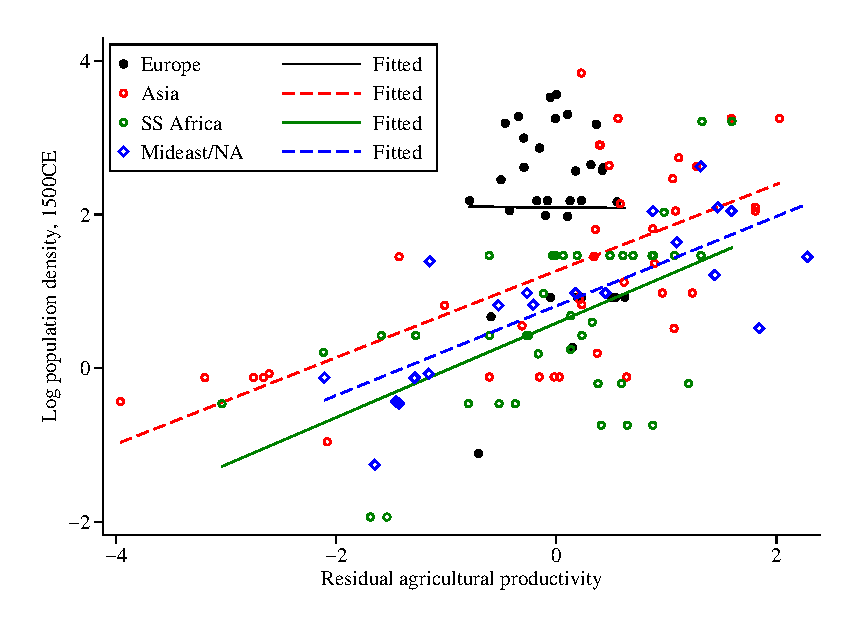
\includegraphics[width=1.0\textwidth]{fig_ag_regions.eps}
\end{center}
\end{figure}

\begin{figure}[htbp]
\begin{center}
\caption{Urbanization and Population Density, by Region, 1500CE}
\label{FIG_ag_urban}
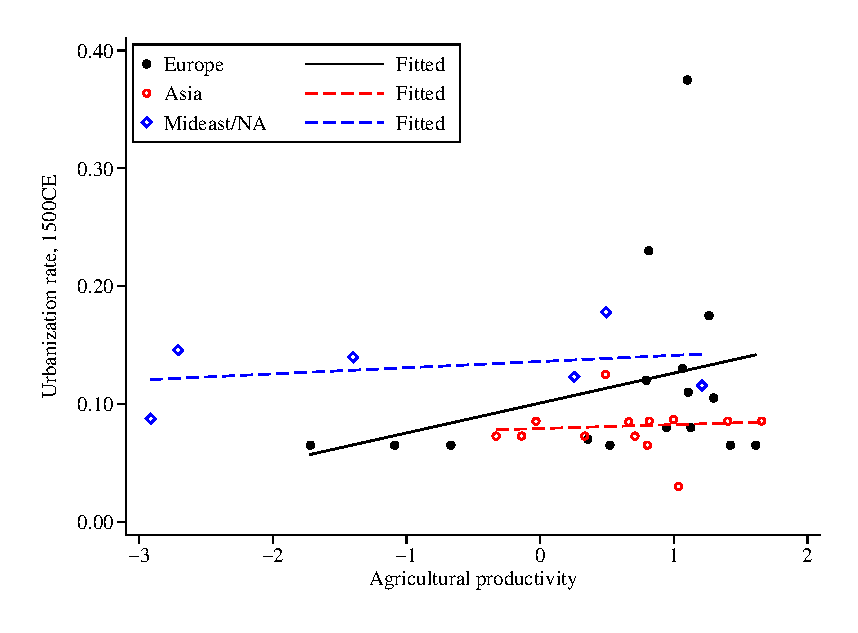
\includegraphics[width=1.0\textwidth]{fig_ag_urban.eps}
\end{center}
\end{figure}


\begin{table}[htb]
\begin{center}
\caption{Relationship of Population Density and Agricultural Productivity, by Region, 1500CE}
\label{TAB_ag_regions}
Log Land Productivity&       0.533&      -0.013&       0.558&       0.615&       0.583&       0.324\\
                    &     (0.059)&     (0.427)&     (0.062)&     (0.116)&     (0.070)&     (0.308)\\
\midrule
Observations        &         147&          33&          40&          39&          21&          25\\
Adjusted R-square   &        0.67&        0.39&        0.65&        0.71&        0.80&        0.46\\

\end{center}
\end{table}

\end{document}